\section{Búsquedas de Artículos}
En la base de datos de \cite{dataDrive} hay 7777 papers. Para las búsquedas se requiere que los papers cuenten con autor, topic profile y venue. Los papers que no cuentan con esos datos, no se tuvieron en cuenta para las búsquedas. De los primeros resultados obtenidos se pudieron observar dos comportamientos no deseados, \textit{soluciones similares para distintos gammas} y \textit{Soluciones con bundles con un solo elemento} a continuación se explicará con más detalle estas soluciones.
\subsection{Soluciones similares para distintos gammas}
De los resultados obtenidos se destacó que el valor de la función objetivo era muy cercano al máximo y que para todos los gammas los resultados eran muy similares. Del análisis que se realizó a los resultados, se detectó que los bundles contenían en su mayoría artículos de un solo tópico. Por lo tanto el intra de los bundles generados es el máximo y así también la distancia con los otros bundles.\\
Al haber tantos artículos con un solo tópico, los resultados que se generan no permiten realizar una correcta comparación de las heurísticas. Por lo tanto a fines de comparar las implementaciones generadas y obtener resultados más interesantes, se decidió no tener en cuenta a los artículos con un solo tópico.
\subsection{Soluciones con bundles unitarios}
Los resultados de las búsquedas en las que se prioriza el inter, se generaban muchos bundles de uno o de dos elementos. Este comportamiento no era el deseado porque no se utilizaba todo el presupuesto.\\
Esto sucede porque en la etapa de generación de bundles de PAC. En el caso que los artículos $A_1$, $A_2$, $A_3$, $A_4$ y $A_5$ con distribución del tópico $t$ mayor a 0.7 y el venue de $A_1$ es $V_1$, de $A_2$ es $V_2$ y de  $A_3$, $A_4$ y $A_5$ es $V_3$. Al generarse los bundles de manera jerárquica, puede darse que en un paso existan el bundle $B_1$ con los artículos $A_1$ y $A_3$ el $B_2$ con $A_2$ y $A_4$ y $B_3$ con $A_5$. Con esta configuración no se pueden juntar los bundles porque se estaría violando la regla de la complementariedad, pero se podría haber generado un bundle con mayor intra si estaría un artículo de cada venue por ejemplo un bundle que con $A_1$, $A_2$ y $A_3$. \\
Para optimizar la generación de los bundles fue por lo que se propuso realizar la búsqueda tabú al finalizar la etapa del Produce.
\subsection{Resultados}
De todos los algorimos descriptos en las secciones anteriores las pruebas realizadas fueron usando {EfficientHAC}, \texttt{Búsqueda Golosa} y \texttt{BOBO} y al terminar su ejecución se aplicó una búsqueda Tabú para intentar mejorar la solución obtenida.\\
\Solucion
{}
{\texttt{EfficientHAC}, \texttt{Búsqueda Golosa} y \texttt{BOBO}}
{simple (no aplica a la búsqueda local)}
{$\in$ $(0,1; 0,3; 0,5; 0,7; 0,9)$}
{10}
{5}
Como primera observación podemos ver la cantidad de bundles que se generan para cada algoritmo de 
producción:\\
\begin{table}[h]
  \centering
  \resizebox{0.5\textwidth}{!} {
    \begin{tabular}{|lc|}
    \hline
    Algoritmo & Bundles Generados \\
    \hline
    EfficientHAC & $2378$ \\
    Greedy & $10$ \\
    BOBO & $100$ \\
    \hline
    \end{tabular}
  }
    \caption {Cantidad de bundles generados antes de la selección final}
\end{table}

\subsubsection{HAC}
\begin{figure}[H]
  \centering
    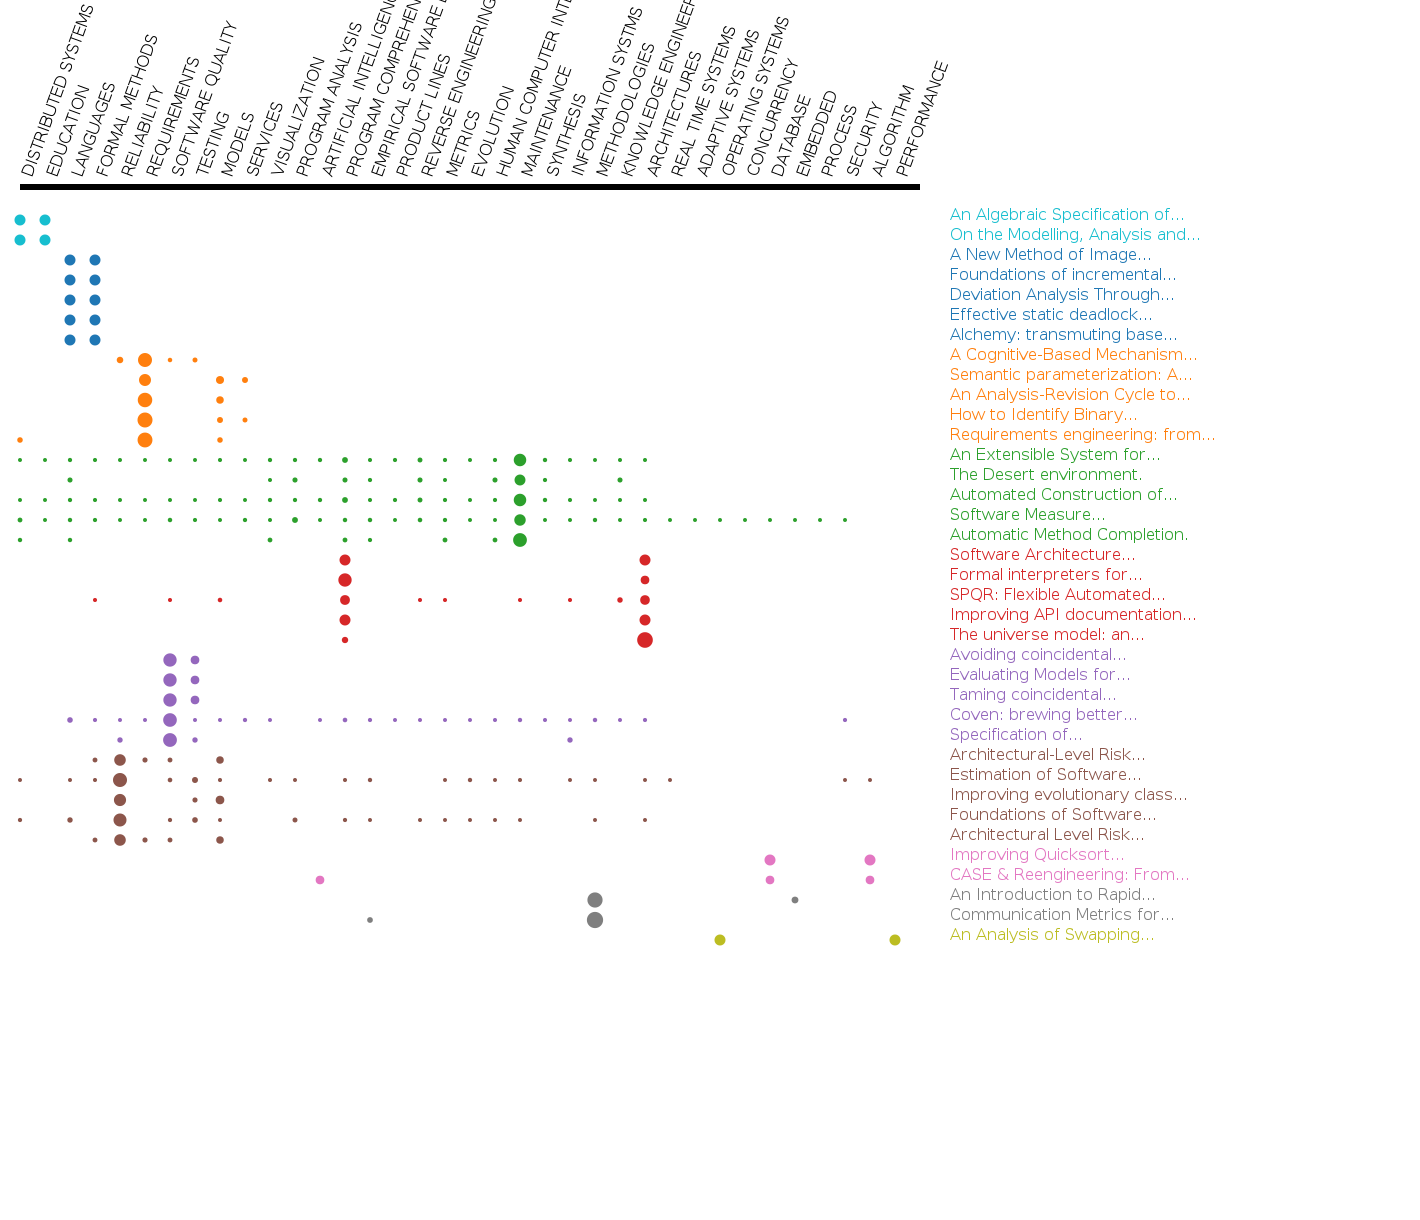
\includegraphics[width=0.8\textwidth]{resultados/papers/HAC/INTRA_INTER/gamma-01.png}
  \caption{Distribución de los perfiles por paper y bundle $\gamma$ = $0.1$ y HAC - Intra Inter}
  \label{res:img-papers-gamma01-hac-intra-inter}
\end{figure}

\begin{figure}[H]
  \centering
    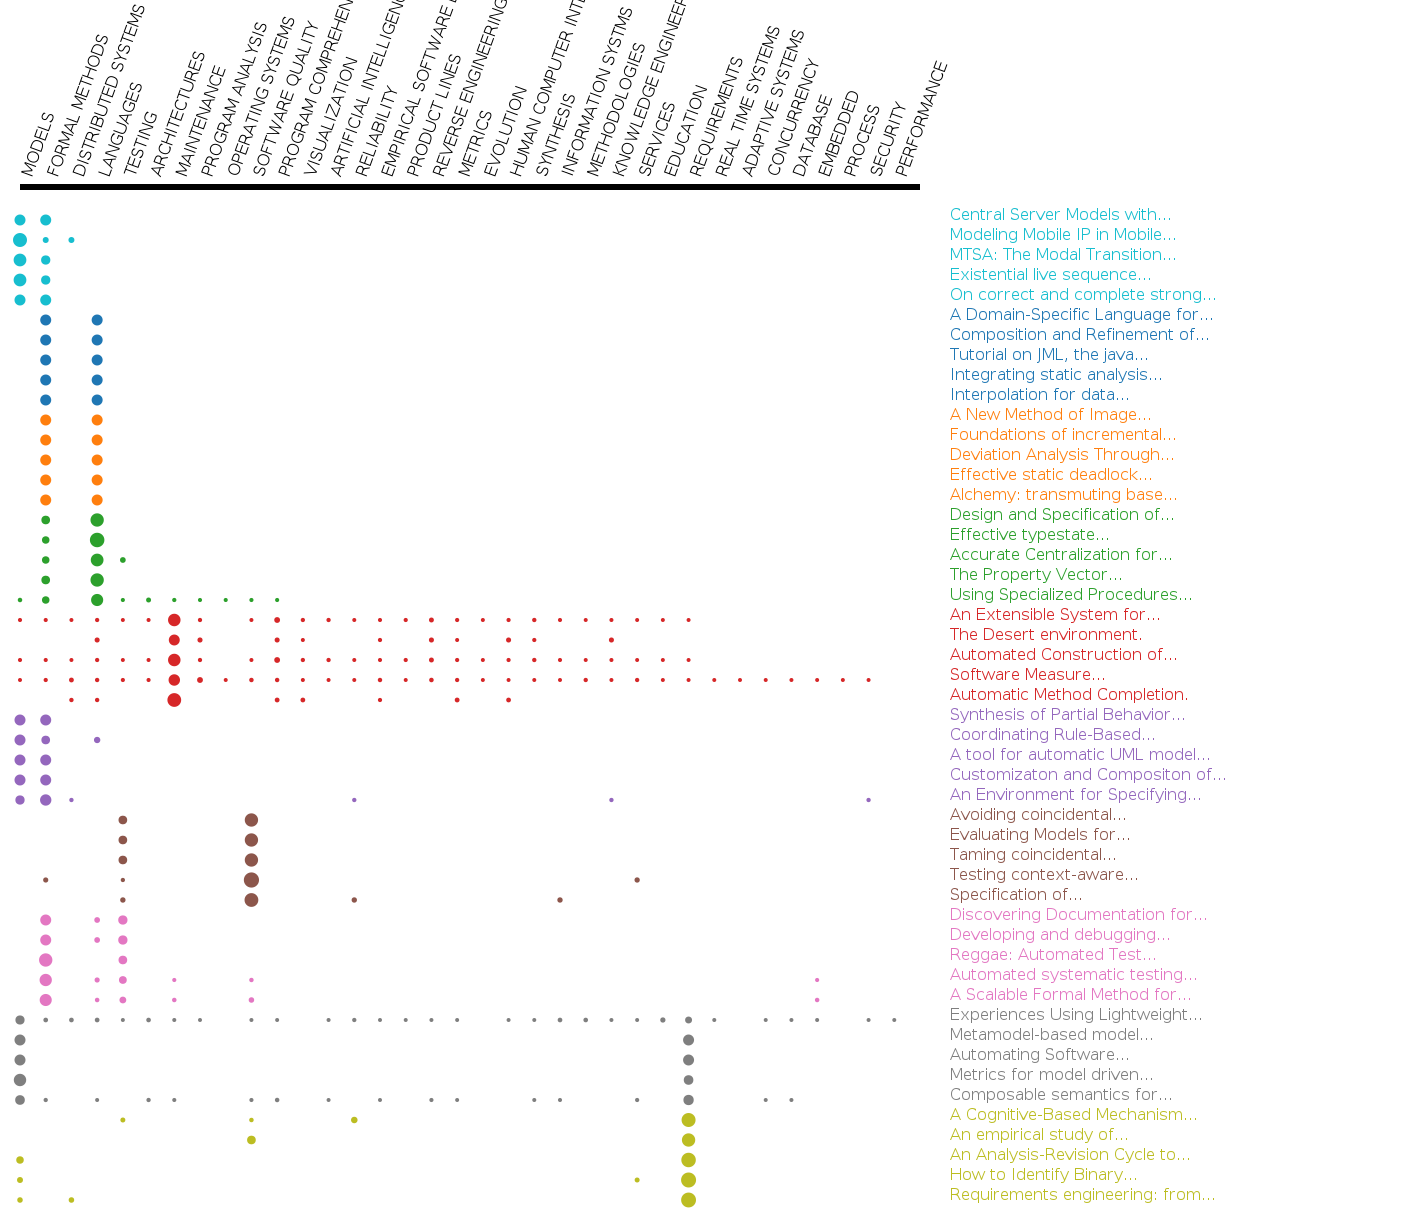
\includegraphics[width=0.8\textwidth]{resultados/papers/HAC/INTRA_INTER/gamma-09.png}
  \caption{Distribución de los perfiles por paper y bundle $\gamma$ = $0.9$ y HAC - Intra Inter}
  \label{res:img-papers-gamma09-hac-intra-inter}
\end{figure}

\begin{figure}[H]
  \centering
    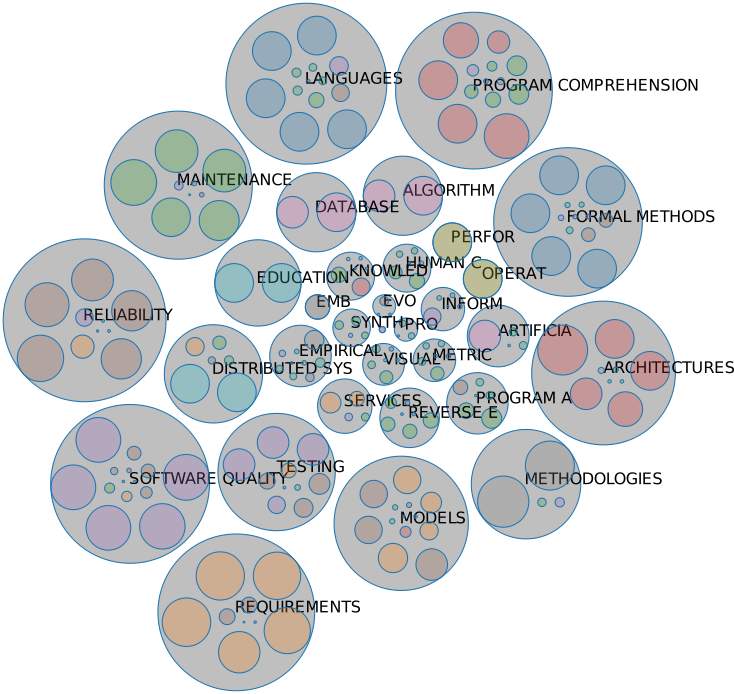
\includegraphics[width=0.8\textwidth]{resultados/papers/HAC/INTRA_INTER/bubbles-gamma-01.png}
  \caption{Distribución de los papers por perfil $\gamma$ = $0.1$ y HAC - Intra Inter}
  \label{res:img-papers-bubbles-gamma01-hac-intra-inter}
\end{figure}

\begin{figure}[H]
  \centering
    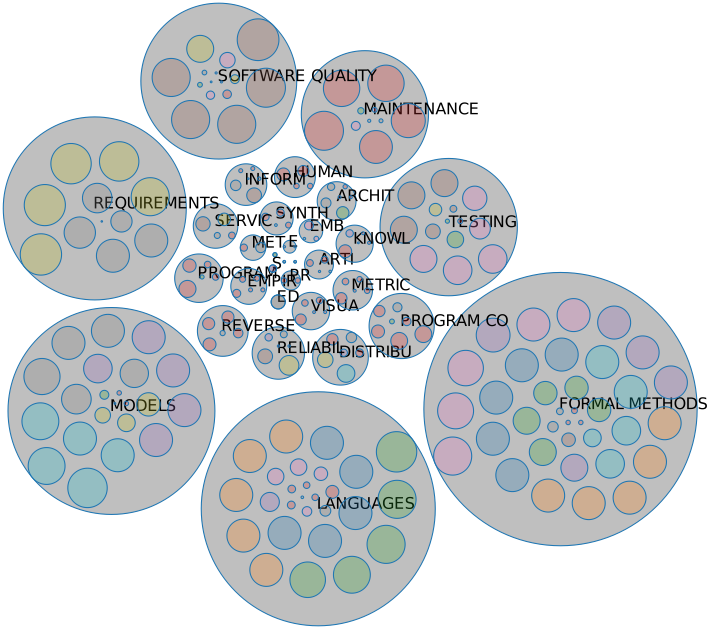
\includegraphics[width=0.8\textwidth]{resultados/papers/HAC/INTRA_INTER/bubbles-gamma-09.png}
  \caption{Distribución de los papers por perfil $\gamma$ = $0.9$ y HAC - Intra Inter}
  \label{res:img-papers-bubbles-gamma09-hac-intra-inter}
\end{figure}

\subsubsection{BOBO}
\begin{figure}[H]
  \centering
    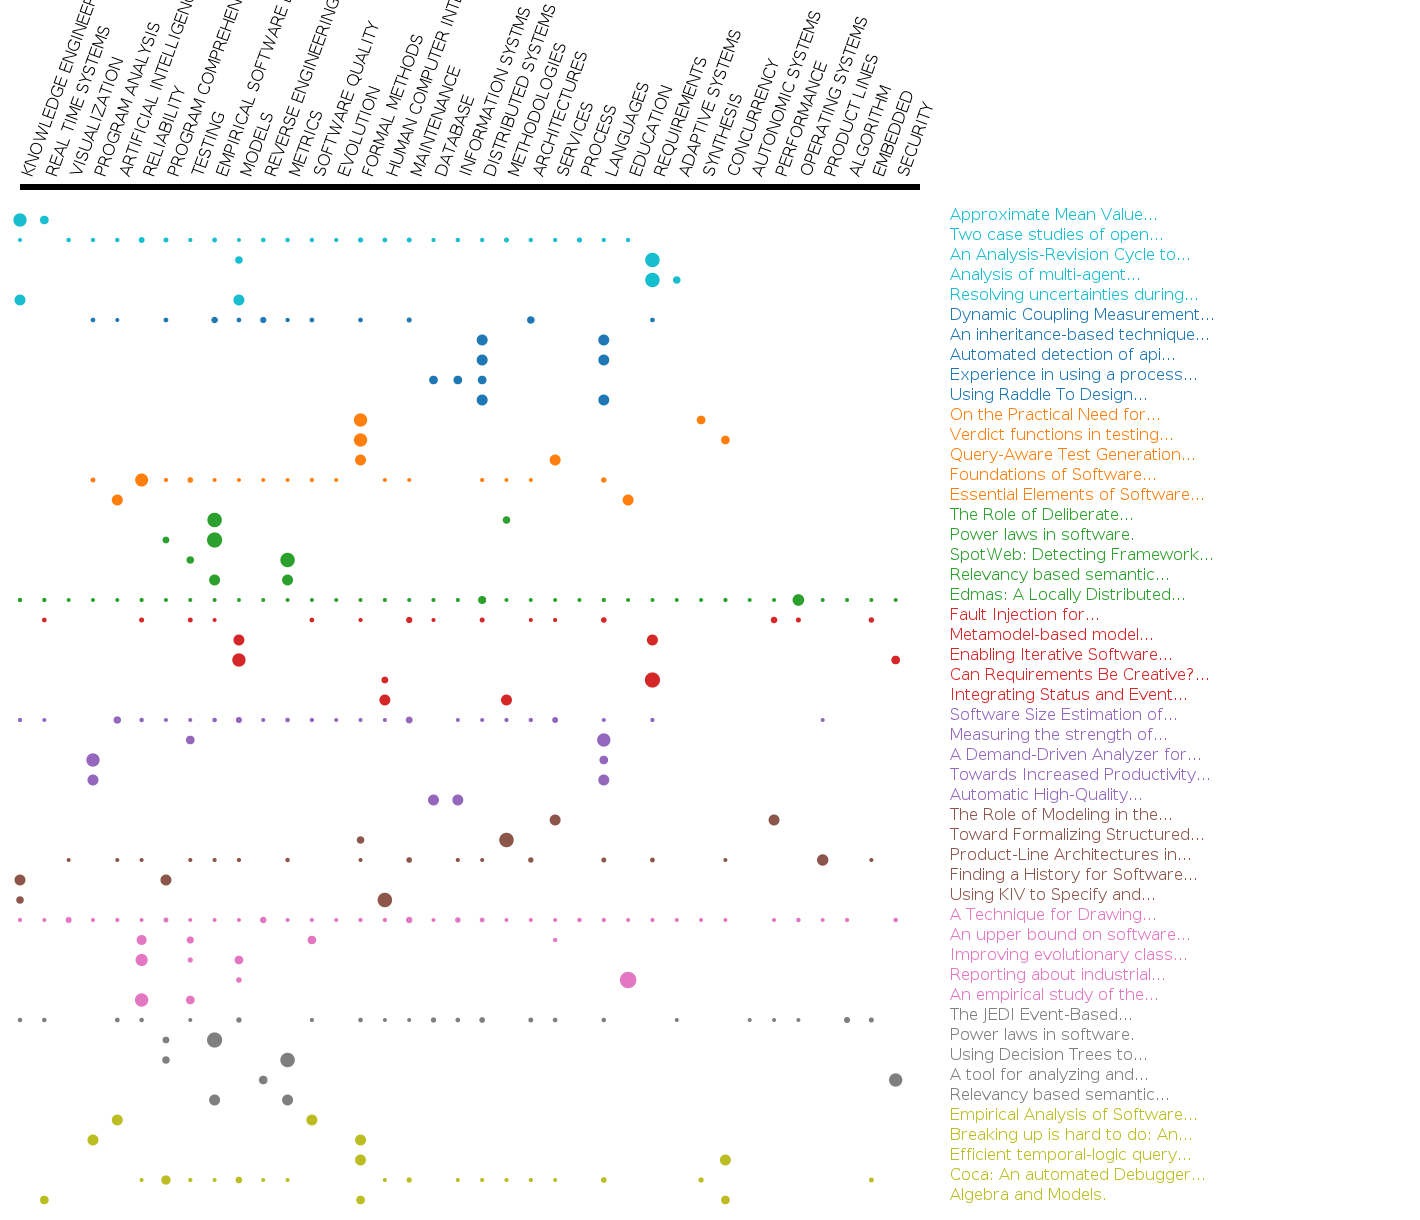
\includegraphics[width=0.8\textwidth]{resultados/papers/BOBO/INTRA_INTER/gamma-01.png}
  \caption{Distribución de los perfiles por paper y bundle $\gamma$ = $0.1$ y BOBO - Intra Inter}
  \label{res:img-papers-gamma01-bobo-intra-inter}
\end{figure}

\begin{figure}[H]
  \centering
    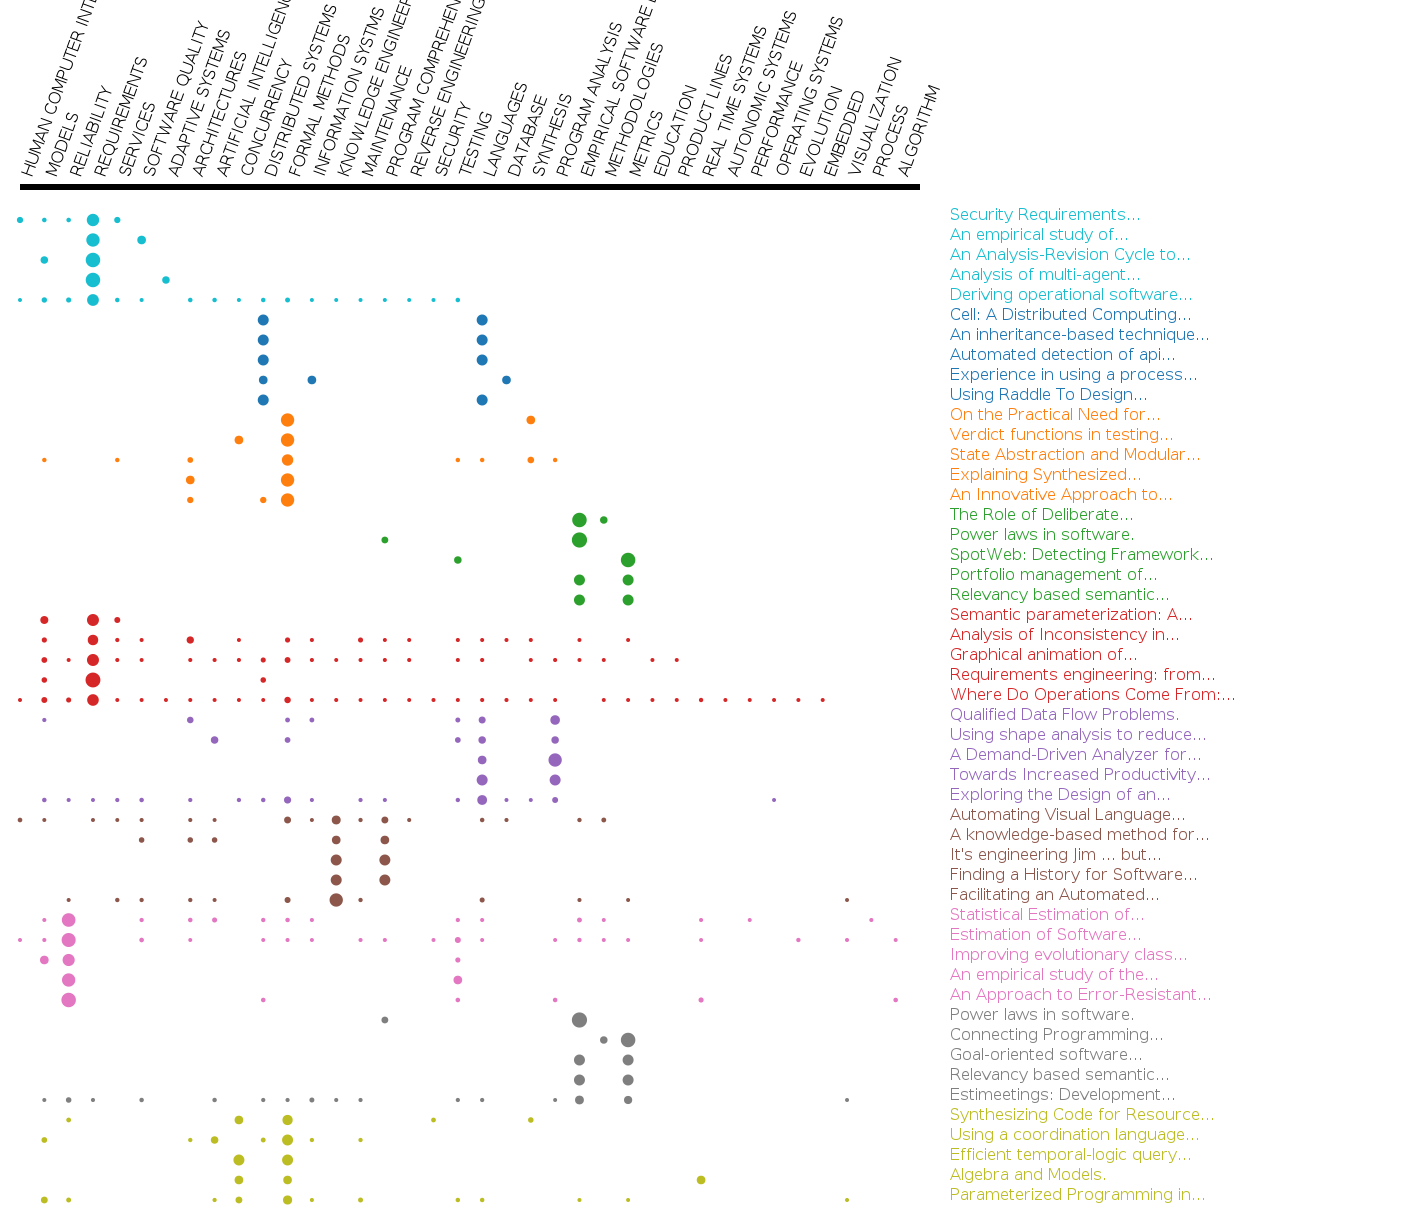
\includegraphics[width=0.8\textwidth]{resultados/papers/BOBO/INTRA_INTER/gamma-with-local-01.png}
  \caption{Distribución de los perfiles por paper y bundle $\gamma$ = $0.1$ y BOBO - Intra Inter con búsqueda Tabú}
  \label{res:img-papers-gamma01-bobo-intra-inter-tabu}
\end{figure}

\begin{figure}[H]
  \centering
    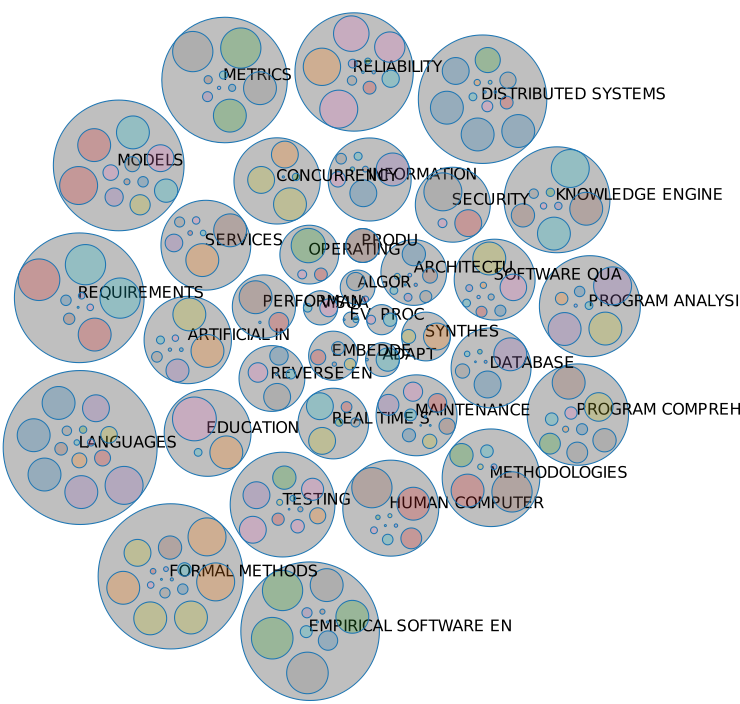
\includegraphics[width=0.8\textwidth]{resultados/papers/BOBO/INTRA_INTER/bubbles-gamma-01.png}
  \caption{Distribución de los papers por perfil $\gamma$ = $0.1$ y BOBO - Intra Inter}
  \label{res:img-papers-bubbles-gamma01-bobo-intra-inter}
\end{figure}

\begin{figure}[H]
  \centering
    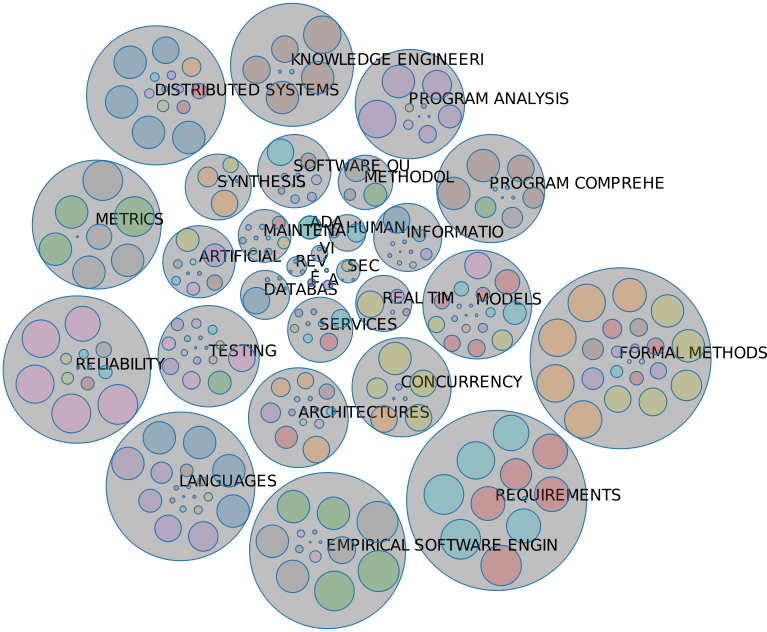
\includegraphics[width=0.8\textwidth]{resultados/papers/BOBO/INTRA_INTER/bubbles-gamma-with-local-01.png}
  \caption{Distribución de los papers por perfil $\gamma$ = $0.1$ y BOBO - Intra Inter con búsqueda Tabú}
  \label{res:img-papers-bubbles-gamma01-hac-intra-inter-bobo}
\end{figure}

\begin{figure}[H]
  \centering
    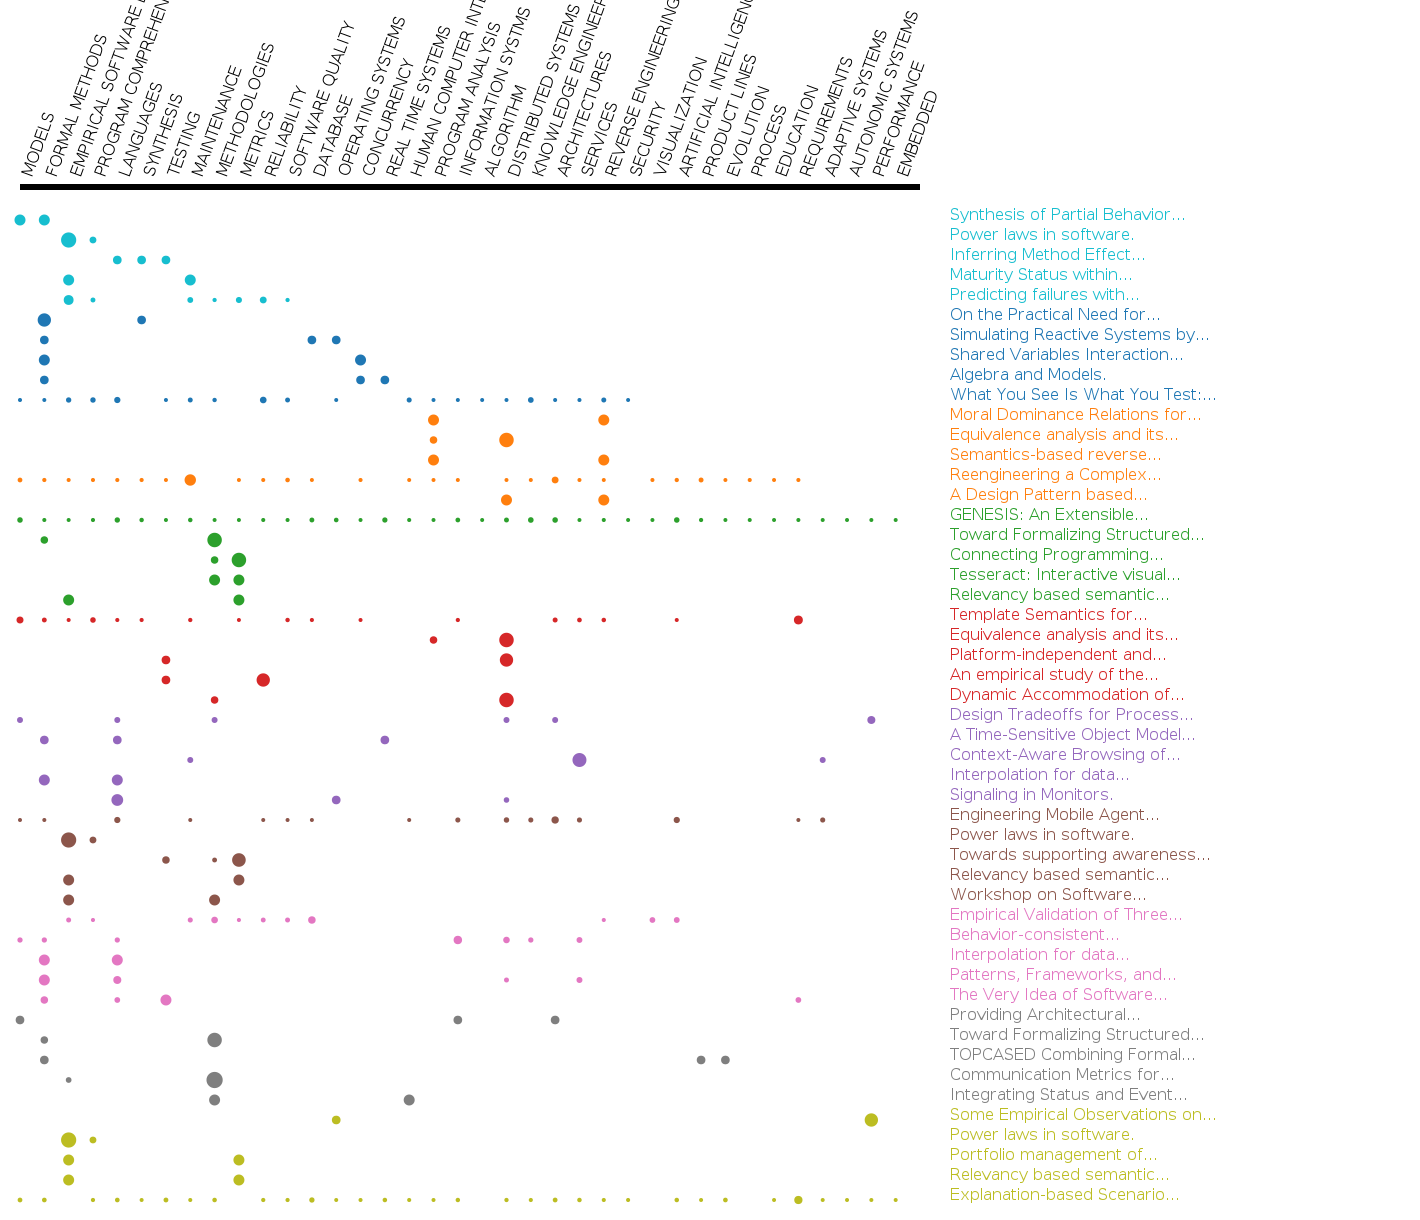
\includegraphics[width=0.8\textwidth]{resultados/papers/BOBO/INTRA_INTER/gamma-09.png}
  \caption{Distribución de los perfiles por paper y bundle $\gamma$ = $0.9$ y BOBO - Intra Inter}
  \label{res:img-papers-gamma09-bobo-intra-inter}
\end{figure}

\begin{figure}[H]
  \centering
    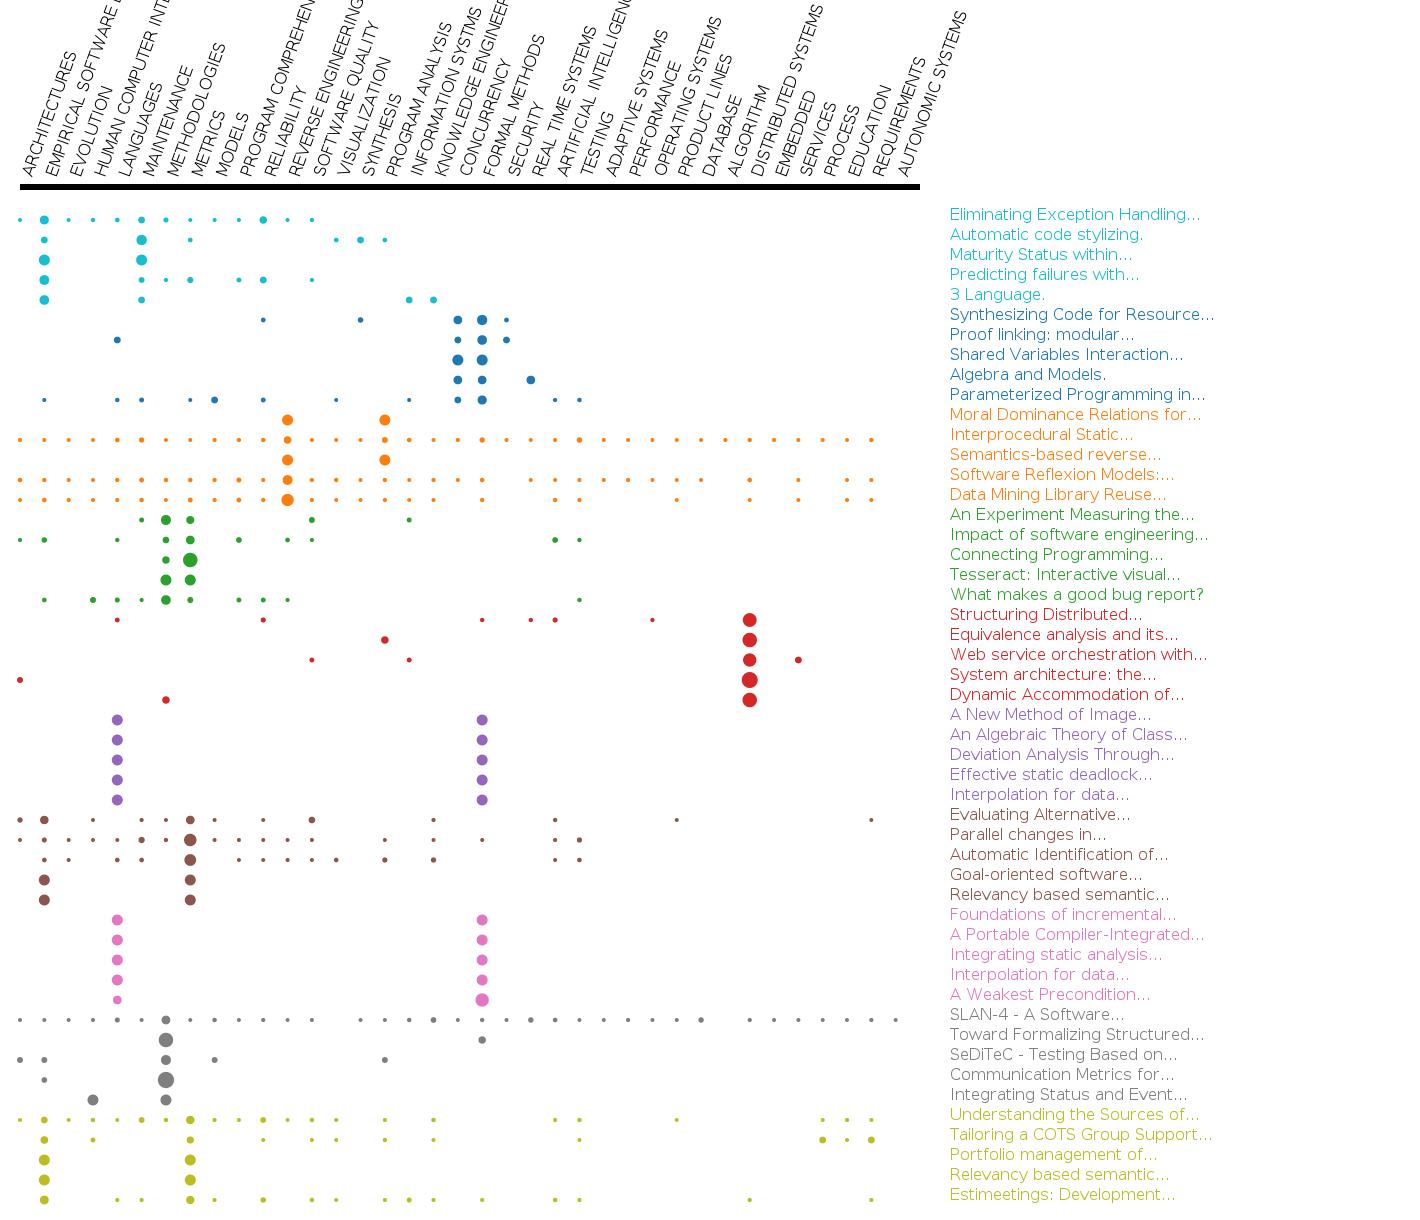
\includegraphics[width=0.8\textwidth]{resultados/papers/BOBO/INTRA_INTER/gamma-with-local-09.png}
  \caption{Distribución de los perfiles por paper y bundle $\gamma$ = $0.9$ y BOBO - Intra Inter con búsqueda Tabú}
  \label{res:img-papers-gamma09-bobo-intra-inter-tabu}
\end{figure}

\begin{figure}[H]
  \centering
    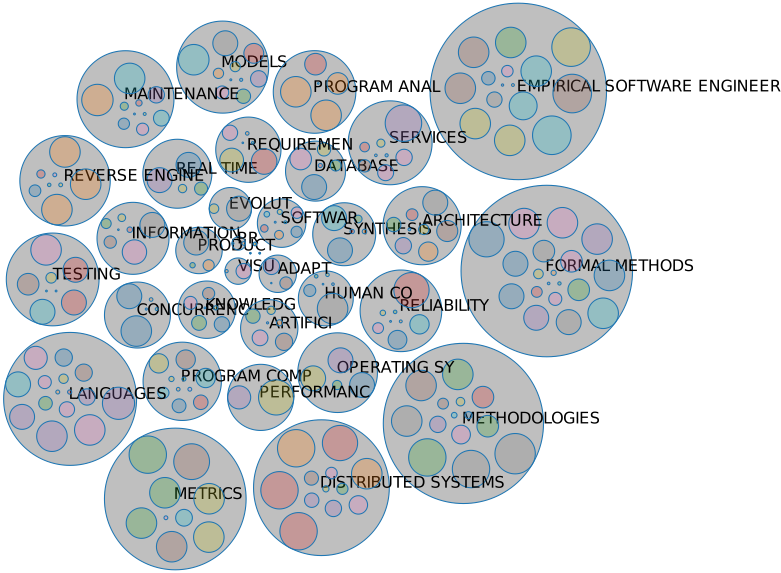
\includegraphics[width=0.8\textwidth]{resultados/papers/BOBO/INTRA_INTER/bubbles-gamma-09.png}
  \caption{Distribución de los papers por perfil $\gamma$ = $0.9$ y BOBO - Intra Inter}
  \label{res:img-papers-bubbles-gamma09-bobo-intra-inter}
\end{figure}

\begin{figure}[H]
  \centering
    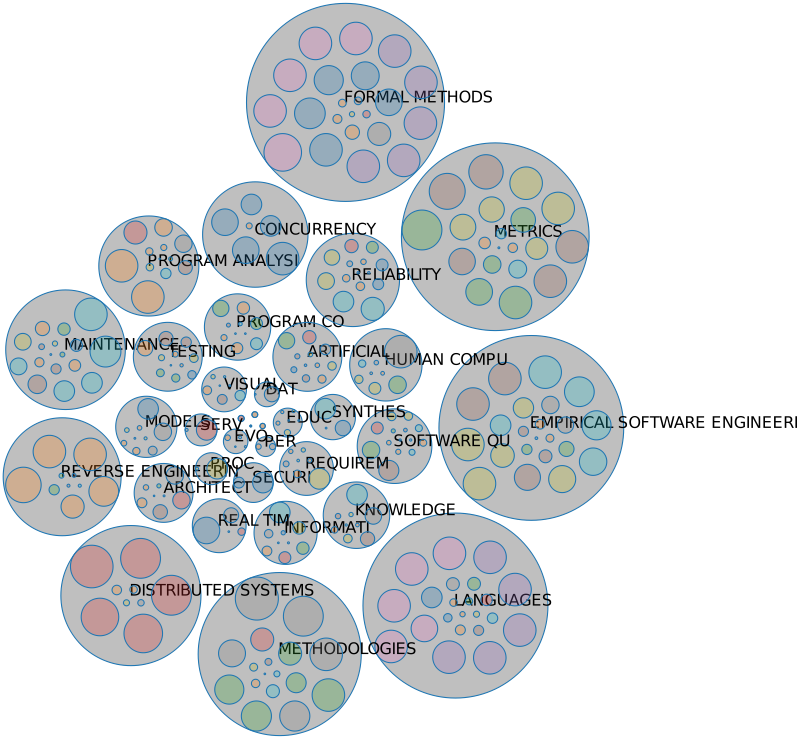
\includegraphics[width=0.8\textwidth]{resultados/papers/BOBO/INTRA_INTER/bubbles-gamma-with-local-09.png}
  \caption{Distribución de los papers por perfil $\gamma$ = $0.9$ y BOBO - Intra Inter con búsqueda Tabú}
  \label{res:img-papers-bubbles-gamma09-hac-intra-inter-bobo}
\end{figure}

En los siguientes gráficos \ref{res:img-papers-agr-gamma01} y \ref{res:img-papers-agr-gamma09} se muestran agrupados por algoritmo de resolución las diferentes estrategias usadas en cada caso y los valores de la función objetivo alcanzado.

\begin{figure}[H]
  \centering
    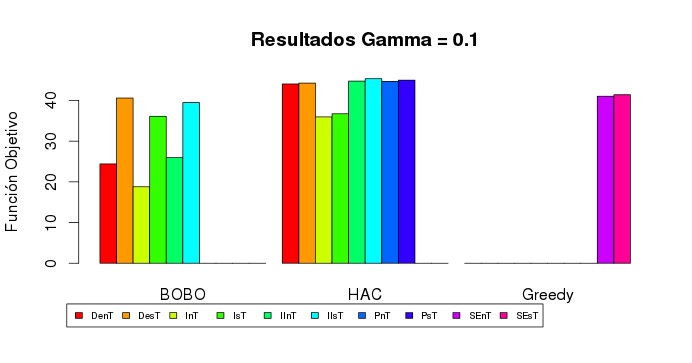
\includegraphics[width=0.8\textwidth]{resultados/papers/Graficos_agrupados/gamma01.png}
  \caption{Función Objetivo $\gamma$ = $0.1$ vs Algoritmos de resolución}
  \label{res:img-papers-agr-gamma01}
\end{figure}

\begin{figure}[H]
  \centering
    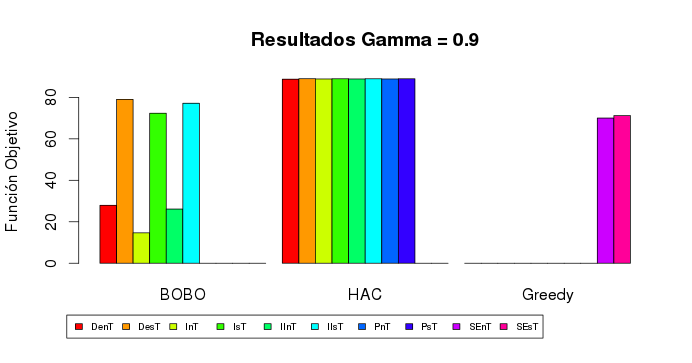
\includegraphics[width=0.8\textwidth]{resultados/papers/Graficos_agrupados/gamma09.png}
  \caption{Función Objetivo $\gamma$ = $0.9$ vs Algoritmos de resolución}
  \label{res:img-papers-agr-gamma09}
\end{figure}

\section{Autores}
\colorbox{red}{RE HACER DE ACA EN ADELANTE}\\
Se generaron soluciones con las siguientes características:\\
\Solucion
{}
{simple y proporcional}
{\texttt{SingleHAC}, \texttt{EfficientHAC} y \texttt{Greedy}}
{$\in$ $(0,1; 0,3; 0,5; 0,7; 0,9)$}
{10}
{5}

En los siguientes gráficos se visualiza los resultados obtenidos para $\gamma$ 0.1 y 0.9. Cada 
nodo representa un bundle y los ejes el valor de la similitud entre cada uno de ellos. La línea más 
gruesa indica un mayor grado de similitud. En cuanto a los vértices al acercarse al azul el valor 
de la intra es menor y al rojo mayor.


Tanto para las soluciones generadas por \texttt{SingleHAC} como por \texttt{EfficientHAC} y con 
cualquier estrategia de selección, todas las soluciones formaron los mismos bundles a pesar de la 
variación del parámetro $\gamma$. Esto se puede ver en los gráficos ya que todos los bundles 
tienen el mayor valor posible para la similitud intra y ningún bundle tiene relación con el 
resto.\\
En parte se debe a que existen $40000$ relaciones de similitud con valor uno. Con la 
heurística Produce and Choose, al momento de producir no se tiene en cuenta el $\gamma$ por lo tanto 
para todos los $\gamma$ en la etapa de producción se producen los mismos bundles.\\
Se realizaron otras búsquedas de soluciones, excluyendo a cinco de los autores que se encuentran 
presentes en todas las soluciones. Pero aún de esta manera en los nuevos resultados obtenidos se 
repite el mismo comportamiento que antes.\\
Además como veremos en \ref{conc:compDifAlgo} los resultados para las ejecuciones con los 
algoritmos jerárquicos se encuentran en los óptimos.
%Por otro lado todas las soluciones generadas por el algoritmo \texttt{HAC} prácticamente no 
%comparten bundles similares con las demás soluciones, ni siquiera autores similares en toda la 
%solución.

\section{Búsqueda con perfil específico}
En una primera aproximación para realizar esta búsqueda solo se modifico la generación de bundles, 
lo cuál, si bien generó resultados diferentes al algoritmo original, no se veía reflejado en los 
resultados las temáticas de los bundles con la elegida para la búsqueda.\\
A partir de ello se decidió modificar también la selección de los bundles para intentar obtener 
bundles relevantes con el perfil elegido.\\
A continuación mostramos la temáticas obtenidas para una búsqueda con un perfil específico de 
ALGORITHM = 50 \%, DISTRIBUTED SYSTEMS = 25 \% y KNOWLEDGE ENGINEERING = 25 \% para la ejecución 
del algoritmo SingleHAC con $\gamma$ = 0.1 y $\gamma$ = 0.9.